%!TEX root=../oi-magistr-si.tex
\section[TVS - Chyby,optimalizace testů,test. automatů]{Kategorizace SW chyb, optimalizace návrhu testů. Testování automatů.}

SW chyba je prezentace toho, že program dělá něco nepředpokládaného. Je to míra toho, kdy program přestává být užitečný (lidem). Je to nesouhlas mezi programem a jeho specifikací (pouze tehdy, jestliže specifikace existují a jsou správné!).

\begin{figure}[h!]
\centering
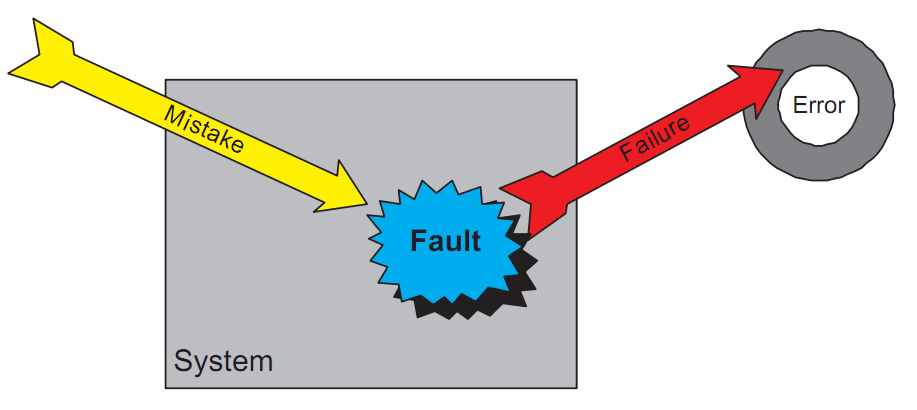
\includegraphics[width=80mm]{13/images/chyba}
\end{figure}

\begin{itemize}[itemsep=0px]
\item \textbf{Pochybení}: Akce člověka, která produkuje nesprávný výsledek.
\item \textbf{Vada}: Nesprávný krok, proces nebo definice dat v počítačovém programu. Výsledek pochybení. Potenciálně vede k selhání.
\item \textbf{Selhání}: Nesprávný výsledek. Projev vady.
\item \textbf{Chyba}: Kvantitativní vyjádření toho, na kolik je výsledek nesprávný
\end{itemize}

\subsection{Kategorie SW chyb}

\begin{itemize}[itemsep=0px]
\item \hl{Chyby UI} - vstupy (nápověda), výstupy (rychlost odezvy)
\item \hl{Chyby omezení} - výjimky, výpočetní chyby
\item \hl{Procesní chyby} - chyba při první inicializaci, zátěž, souběh více vláken
\item \hl{Chyby vedení} - stará verze knihovny, slabá doc
\item \hl{Chyby požadavků, vlastností a funkčnosti} - neúplné, nejednoznačné
\item \hl{Strukturální chyby} - logika (neporozumění log. operátorům), GOTO, konverze typů
\item \hl{Datové chyby} - specifikace objektů
\item \hl{Chyby implementace} - syntaktické chyby, chyby paměti, hranice pole
\end{itemize}
\paragraph{Chyby uživatelského rozhraní}
\begin{itemize}[itemsep=0px]
\item Problémy s funkčností - program nedělá něco, co by měl dělat nebo to dělá nevhodně (zmatečně, neúspěšně), lze některé operace provést obtížně.
\item To co se \uv{předpokládá} od programu, žije pouze v mysli uživatele
\item Všechny programy mají problémy s funkčností vzhledem k různým uživatelům.
\item Funkční problém je chybou, pokud očekávání uživatele jsou rozumná.
\item \textbf{Vstupy}

    \begin{itemize}[itemsep=0px]
    \item Jak lze nalézt, jak program používat (jaká je nápověda)?
    \item Jak snadné je ztratit se v programu?
    \item Jaké chyby uživatel dělá a kolik ho to stojí času?
    \item Co mu chybí?
    \item Nutí prg. uživatele přemýšlet nepřirozeně?
    \end{itemize}
    
\item \textbf{Výstupy}

    \begin{itemize}[itemsep=0px]
    \item Rychlost je základ interaktivního sw.
    \item Cokoli co budí dojem pomalého prg. je problém.
    \item Získá uživatel, co potřebuje?
    \item Mají výstupy smysl?
    \item Může uživatel přizpůsobit výstup potřebám?
    \item Zle výstup přesměrovat dle potřeby(monitor, tisk, soubor, $\hdots$)?
    \end{itemize}
\end{itemize}
\paragraph{Chyby omezení}

\begin{itemize}[itemsep=0px]
\item Chyby zpracování vyjímek zahrnující neschopnost
    \begin{itemize}[itemsep=0px]
    \item Předvídání možnosti chyby a bránit se jim
    \item Zpracování podmínek chyby
    \item Zpracovaní detekované chyby různými způspby
    \end{itemize}
\item Chyby hraničních podmínek
    \begin{itemize}[itemsep=0px]
    \item Nejjednodušší hranice jsou numerické
    \item Mezní nároky na paměť, za kterých program může pracovat
    \end{itemize}
\item Výpočetní chyby
    \begin{itemize}[itemsep=0px]
    \item Chyby aritmetiky jsou časté a obtížně detekovatelné
    \item Program ztrácí přesnost během výpočtu vlivem zaokrouhlovacích chyb a ořezání
    \item Výpočetní chyby způsobené chybnými algoritmy
    \end{itemize}
\end{itemize}

\paragraph{Procesní chyby}
\begin{itemize}[itemsep=0px]
\item Sekvenční
    \begin{itemize}[itemsep=0px]
    \item Počáteční a jiné speciální stavy
        \begin{itemize}[itemsep=0px]
        \item Funkce mohou selhat při prvním použití, např. chybějící inicializační informace či soubory
        \item Nastaví se skutečně vše do výchozího bodu, vymažou se všechna data, jestliže uživatel provede reset programu?
        \end{itemize}
    \item Chyby řízení nastane, pokud program provede chybný příští krok
        \begin{itemize}[itemsep=0px]
        \item Extrémní chyba nastane, pokud se program zastaví nebo vymkne kontrole řízení
        \end{itemize}
    \end{itemize}
\item Paralelní
    \begin{itemize}[itemsep=0px]
    \item Chyby souběhu - race error
        \begin{itemize}[itemsep=0px]
        \item Jedny z nejméně testovaných
        \item Nastávají v multiprocesových sys. a integračních sys.
        \item Velmi obtížně se opakují
        \end{itemize}
    \item Zátěžové podmínky
        \begin{itemize}[itemsep=0px]
        \item Program se začne chovat chybně pokud se přetíží
            \begin{itemize}[itemsep=0px]
            \item Chyby velkého objemu - hodně práce za dlouhou dobu
            \item Chyby velkého stresu - hodně práce v daném okamžiku
            \end{itemize}
        \item Všechny programy mají své limity, ale je důležité vědět co nastane
        \end{itemize}
    \end{itemize}
\end{itemize}

\paragraph{Chyby vedení}
\begin{itemize}[itemsep=0px]
\item Hardware - program posílá chybová data na zařízení, ignorují chybové kódy přicházející zpět a zkouší použít zařízení, která neexistují nebo jsou aktuálně vytížená
\item Řízení zdrojů a vedení
    \begin{itemize}[itemsep=0px]
    \item Staré problémy se opět objevují, pokud programátor zakomponuje do programu nějakou starou verzi komponenty
    \item Ujistěte se, že program má správný copyright, vstupní obrazovky a
    \end{itemize}čísla verzí
\item Dokumentace - slabá dokumentace může způsobit ztrátu víry uživatele, že sw. pracuje spráně
\item Chyby testování
    \begin{itemize}[itemsep=0px]
    \item Chyby udělané testy jsou nejčastějšími chybami objevenými během testování
    \item Jestliže program navádí většinu uživatelů ke způsobení chyb, pak je špatně navržen
    \end{itemize}
\end{itemize}
    
\paragraph{Chyby požadavků, vlastností a funkčnosti}

\begin{itemize}[itemsep=0px]
\item Požadavky a specifikace
    \begin{itemize}[itemsep=0px]
    \item Neúplné, nejednoznačné, vzájemně si odporující
    \item Hlavní zdroj drahých chyb
    \end{itemize}
\item Chyby vlastností - chybějící, chybné, nevyžádané vlastnosti
\item Interakce vlastností - nepredikované interakce(přesměrování telefonu ve smyčce)
\item Preventivní opatření proti chybám ve specifikacích a vlastnostech:
    \begin{itemize}[itemsep=0px]
    \item Problém v komunikaci člověk-člověk
    \item Jazyk formálních specifikací poskytující krátkodobé řešení, avšak neřeší problém chyb v dlouhodobém horizontu.
    \end{itemize}
\end{itemize}
    
\paragraph{Strukturální chyby}
\begin{itemize}[itemsep=0px]
\item Chyby v řízení sekvencí
    \begin{itemize}[itemsep=0px]
    \item Příkaz GOTO
    \item Většina chyb řízení (v novém kódu) se dá snadno testovat a je chycena během testování jednotek
    \item Neupravený starý kód může mít řadu chyb v řídicím toku
    \item Stlačování za účelem kratšího prováděcího času nebo menšího nároku na paměť je špatná politika
    \end{itemize}    
\item Chyby zpracování
    \begin{itemize}[itemsep=0px]
    \item Zahrnuje chyby vyhodnocení aritmetických, algebraických nebo matematických fcí. a výběr algoritmu
    \item Řada problému vznikne špatnou konverzí dat na jinou reprezentaci
    \end{itemize}
\item Chyby logiky
    \begin{itemize}[itemsep=0px]
    \item Neporozumění jak se selekční či logické operátory chovají samostatně nebo v kombinacích
    \item Neporozumění sémantice uspořádání logických výrazů a jeho vyhodnocení specifickými překladači
    \item Chyby datového toku - nevztahují se k chybám řízení
    \item Chyby toku řízení - část logického výrazu, která je použita pro ovládání toku řízení
    \end{itemize}
\item Inicializační chyby - opomenutí inicializace pracovního prostoru, registů, nebo části dat
\item Chyby a anomálie toku dat
    \begin{itemize}[itemsep=0px]
    \item Nastane pokud existuje cesta, při které se udělá s daty něco neodůvodněného např. použití neinicializované proměnné, nebo neexistující proměné
    \item Jsou stejně tak důležité jako anomálie toku řízení
    \end{itemize}
\end{itemize}
    
\paragraph{Datové chyby}
\begin{itemize}[itemsep=0px]
\item Lze je nalézt ve specifikacích datových objektů, jejich formátů, počtu nebo jejich počátečních hodnotách
\item Sw. se vyvíjí k tabulkám obsahujících řídicí a procesní fce.
\item Trendy programování vedou k zvýšenému používání nedeklarovaných, interních, speciálních programovacích jazyků
\item Dynamické vs. statické
    \begin{itemize}[itemsep=0px]
    \item Protože efekt poškození dynamických dat se může projevit velmi vzdáleně od příčiny, nalézají se takovéto chyby velmi obtížně
    \item Základní problém zbytků ve sdílených zdrojích (např. vyčištění po použití uživatelem, sdílené čištění pomocí ovladače zdrojů, žádné čištění)
    \end{itemize}
\item Informace, parametr, řízení
    \begin{itemize}[itemsep=0px]
    \item Údaj plní jednu ze tří rolí: jako parametr, jako řízení, jako zdroj informace
    \item Informace je obvykle dynamická s tendencí lokality pro danou transakci (nedostatek ochranného kódu validace dat)
    \item Neadekvátní validace dat často vede k ukazování prstem
    \end{itemize}
\item Obsah, struktura, atributy
    \begin{itemize}[itemsep=0px]
    \item Obsah - aktuální bitový vzor, řetězec znaků, nebo číslo vložené do datové struktury
    \item Struktura - velikost, tvar a počty popisující datové položky
    \item Atributy - specifikace významu (sémantika)
    \item Základem je explicitní dokumentace obsahu, struktury a atributů všech datových objektů
    \end{itemize}
\end{itemize}

\paragraph{Chyby implementace}
\begin{itemize}[itemsep=0px]
\item Chyby kódování
    \begin{itemize}[itemsep=0px]
    \item Dobrý překladač chytne syntaktické chyby, nedeklarovaná data, procedury, kód a mnoho inicializačních problémů
    \item Častou chybou kódu jsou dokumentační chyby (komentáře)
    \item Úsilí programování je dominováno údržbou
    \end{itemize}
\item Chyby paměti
    \begin{itemize}[itemsep=0px]
    \item Charakteristiky
        \begin{itemize}[itemsep=0px]
        \item Nejobtížnější chyby z hlediska lokalizace
        \item Nejdůležitější chyby z hlediska opravy
        \item Projevy nesprávného obsahu paměti jsou nepredikovatelné
        \item Chyby v obsahu paměti se typicky projevují vzdáleně od jejich příčiny
        \item Chyby zůstávají často nedetekováné dokud nejsou náhodně spuštěny
        \end{itemize}
    \item Typy chyb
        \begin{itemize}[itemsep=0px]
        \item Chyby hranic polí
        \item Přístup přes nedefinovaný ukazatel
        \item Čtení z neinicializované paměti
        \item Chyby ztráty paměti (memory leaks)
        \end{itemize}
    \item Slabá místa výkonnosti
        \begin{itemize}[itemsep=0px]
        \item Kolekce vyčerpávající přesné množiny dat pro výkonnostní test programu a každé jeho komponenty (profilování)
        \item Zaměření se na kritická data
        \item Sběr správně vybraných dat
            \begin{itemize}[itemsep=0px]
            \item Řádka - kolikrát proběhla každá řádka - nejpřesnější, ale nejnáročnější na sběr dat
            \item Funkce - méně podrobné než předchozí
            \item Čas - data se sbírají z údajů časovaných běhů funkcí. Data jsou správná pro daný běh, ale závisí na stavu mikroprocesoru a paměti. Nejméně náročný sběr
            \end{itemize}
        \end{itemize}
    \end{itemize}
\end{itemize}

\subsection{Optimalizace návrhů testů}

Optimalizovat testování chceme za účelem snížení jeho časové náročnosti. Např. u PLC chceme testovat instrukci, která má 5 parametrů a každý z nich může nabývat 17ti hodnot. To je $17^5$ kombinací (1 419 857) tedy cca 230 dnů testování.

V praxi se ale ukázalo, že většina chyb nevzniká při všech 5ti nastavených parametrech, ale při interakci jen několika z nich. Vytvářejí se pak testy, které pokrývají jen všechny možné k-tice (ne všechny kombinace). Pomocí následujících metod se dá počet testovaných případů redukovat.

\subsubsection{Princip párového testování}
Jak již bylo zmíněno, při \textbf{ideálním testovacím plánu} by bylo nutné projít všechny kombinace hodnot parametrů, tj. $1 419 857 = 17^5$ kombinací - 230 dnů testování.


Praktický testovací plán využívá toho, že selhání jsou způsobena interakcí pouze několika parametrů, Proto se provádí testování kombinacemi pokrývající všechny možné k-tice (k-tice komprimovány do plných kombinací).

\paragraph{Příklad}
\begin{itemize}[itemsep=0px]
\item 5 parametrů
\item 17 hodnot pro každý parametr
\item \textbf{Optimalizace:}
\item Nezávislé parametry: 17 kombinací,
\item Počet párů: 5 nad 2 = 10 parametrových párů,
\item Hodnot pro každý pár: $289 = 17^2$ kombinací hodnot pro každý pár,
\item Počet hodnot pro všechny pár: $2890 = 289*10$ párů parametrových hodnot,
\item zredukovaných 289 kombinací obsahující všechny páry,
\item 30 minut testování.
\end{itemize}

\subsubsection{Optimalizace metodou ortogonálních polí}
Ortogonální pole je matice velikosti $m \times n$, ve které při testování parametrických párů jednotlivé sloupce odpovídají faktorům (parametrům funkce, případně jiným hodnotám, na kterých závisí testovací případ) a řádky jednotlivým testovacím případům.

Ortogonální pole jsou označována podle toho, kolik úrovní (významných hodnot) umožňují jednotlivým faktorům. Ortogonální pole $(2^{1} \times 3^{7})$ má celkem 8 faktorů. Jeden faktor může mít dvě významné hodnoty, a sedm dalších může mít až 3 významné hodnoty.

Pro použití této techniky je zapotřebí příklad nejprve zakódovat. Tato procedura je velmi snadná – nejprve nalezneme všechny faktory (parametry příkladu) a zjistíme, kolik mají úrovní. Poté nalezneme vhodné ortogonální pole.

Vybrané pole musí umožňovat alespoň tolik faktorů, kolik má náš případ. Dále je nutné, aby jednotlivé faktory měly dostatečný počet úrovní.

Nyní můžeme přejít k samotnému kódování. Každému parametru naší úlohy přiřadíme jeden sloupec – případné přebytečné sloupce můžeme ignorovat. Každé významné hodnotě přiřadíme jednu úroveň – pokud má sloupec více úrovní než potřebujeme, tak můžeme některé významné hodnotě přiřadit více úrovní, tím tuto hodnotu otestujeme více než ostatní (ale stále platí, že otestujeme každou parametrickou dvojici alespoň jednou).

V tomto okamžiku již můžeme pomocí našeho zakódování číst jednotlivé řádky ortogonálního pole - samotné testovací případy.

Ortogonální pole není jednoduché nalézt, testovací případy musí být balancované atd., proto existují jejich katalogy (pole nekonstruujeme, ale používáme již dostupná pole z katalogů).

\begin{table}[h]
\begin{tabular}{|l|l|l|l|}
\hline
  & 1 & 2 & 3 \\ \hline
1 & 1 & 1 & 1 \\ \hline
2 & 1 & 2 & 2 \\ \hline
3 & 2 & 1 & 2  \\ \hline
4 & 2 & 2 & 1 \\ \hline
\end{tabular}
\vspace{10px}
\caption{Ortogonální pole $L_4 (2^3)$}
\end{table}

\subsubsection{Optimalizace metodou latinských čtverců}


\textbf{Latinský čtverec} je matice s $n$ řádky a $n$ sloupci taková, že každý element obsahuje celé číslo do 1 do $n$ tak, že se v žádném sloupci nebo řádku nevyskytuje žádné číslo vícekrát než jednou.

\textbf{Párově ortogonální latinské čtverce} - každý elment v daném čtverci vystupuje v relaci s každým elementem druhého čtverce právě jedenkrát. Pro jakoukoliv mocninu prvočísla $n$ existuje $n-1$ párově ortogonálních latinských čtverců velikosti $n \times n$.

\begin{itemize}[itemsep=0px]
\item ze zadání se identifikují faktory a úrovně
\item určím počet párově-ortogonálních čtverců jako $N$ = max(faktorů-2, nejvyšší\_úroveň)
\item najdu si čtverce v literatuře, ($N+1$) rozměrné
\item nyní generuji testovací případy: první faktor je číslo řádku, druhý faktor číslo sloupce, další hodnoty podle čísel na souřadnicích v jednotlivých čtvercích
\item vygeneruje mi to $(N+1)^2$ testovacích případů
\end{itemize}

\subsection{Testování automatů}
\hl{Konečný automat je výborný model pro testování aplikací řízených pomocí menu} (ovládání aplikace se provádí pomocí výběru položek z menu).

Vrcholy zobrazují stavy (stav aplikace). Hrany mezi stavy reprezentují vyběr položky menu (a tím přechod do dalšího stavu). Automat by měl být silně souvislý, pokud existují oddělené stavy (izolované), tak tyto stavy zavání chybou, jsou podezřelé (nevede k nim položka v menu).

\vspace{-10px}

\paragraph{Skryté stavy}
Test nelze zahájit, pokud systém není potvrzením způsobem v počátečním stavu. Dát si pozor na skryté stavy. Při testování SW můžeme předpokládat věci, které nemusí obecně platit (např. že víme, ve kterém stavu se systém nachází). Pokud existují skryté stavy tak se typicky nejedna o jeden či dva stavy, ale o celý stavový prostor.

\paragraph{Postup návrhu testů}

\begin{itemize}[itemsep=0px]
\item identifikuj vstupy
\item definuj kódy vstupu
\item idenfikuj stavy
\item definuj kódovaní stavů
\item identifikuj výstupní akce
\item definuj kódování výstupních akcí
\item specifikuj tabulku přechodů a tabulku výstupů - a zkontroluj ji
\item navrhni testy
\item proveď testy
\item pro každý vstup ověř jak přechod tak i výstup
\end{itemize}

Každý test začíná v počátečním stavu. Z počátečního stavu se systém přivede nejkratší cestou k vybranému stavu, provede se zadný přechod a systém se nejkratší možnou cestou přivede opět do počátečního stavu (tzv. okružní cesta).

\paragraph{Formální konstrukce testů}

Nechť $L$ je \textbf{množina vstupních sekvencí} a $q, q'$ dva stavy. $L$ \textbf{rozliší} stav $q$ od $q'$, jestliže existuje sekvence $k$ v $L$ taková, že \textbf{výstup} získaný apikací $k$ na automat ve \textbf{stavu $q$} je \textbf{různý} od \textbf{výstupu} získaný aplikací $k$ na \textbf{stav $q'$}. Chceme minimální automat (tj. takový, který neobsahuje redudantní stavy).

Množina vstupních sekvencí $W$ se nazývá \textbf{charakterizační množina}, jesltiže může rozlišit jakékoliv dva stavy automatu.

\begin{itemize}[itemsep=0px]
\item \textbf{Pokrytí stavů} je množina vstupních sekvencí $L$ taková, že lze nalézt prvek množiny $L$, kterým se lze dostat do jakéhokoliv žádaného stavu z počátečního stavu $q_0$.
\item \textbf{Pokrytí přechodů} minimálního automatu je množina vstupních sekvencí $T$, která je pokrytím stavů a uzavřená z hlediska pravé kompozice s množinou vstupů $Input$.

$$seq \in T = L \bullet (Input \cup {<>})$$

\end{itemize}
